\documentclass[../main.tex]{subfiles}
\begin{document}

\ifSubfilesClassLoaded{
	\mainmatter
	\setcounter{chapter}{3}
}{}

\chapter{Results}
\label{ch:result}
\section{Drell-Yan Cross Section Ratio}
\pdfmargincomment{run 5-6 compared with 2-3 and full data set} 

\subsection{Intensity extrapolation}

\subsection{Mass fit result}

\subsection{Extraction of \texorpdfstring{$\bar{d}/\bar{u}$}{dbar/ubar}}
The $\sigma_{pd}/2\sigma_{pp}$ ratio is used by the NNPDF collaboration in
their PDF extraction\cite{ball2021} and their result is shown in Fig.\
\ref{fig:nnpdf_e906}.

\begin{figure}[htbp!]
	\centering
	\begin{subfigure}{0.45\linewidth}
		\includegraphics[width=\linewidth]{data_vs_theory_nnpdf40_e906}
		\caption{Calculated Drell-Yan cross section ratio.}
		\label{subfig:nnpdf_e906_csr}
	\end{subfigure}
	\begin{subfigure}{0.45\linewidth}
		\includegraphics[width=\linewidth]{placeholder}
		\caption{Extracted $\bar{d/}\bar{u}$ ratio.}
		\label{subfig:nnpdf_e906_x2}
	\end{subfigure}
	\caption{Comparison of NNPDF4.0\cite{ball2021} with the SeaQuest
		result\cite{dove2021}.}
	\label{fig:nnpdf_e906}
	\pdfmargincomment{Should be compared with the new result from run5-6 and full
		data set}
\end{figure}

\section{Charmonium Cross Section}
\pdfmargincomment{absolute cross section and cross section ratios; mean pT for
	jpsi as a function of root s}

	
The massfits in each kinematic bins are shown in 
\cref{fig:massfit_57-70_xF,fig:massfit_5-6_xF,fig:massfit_57-70_pT,fig:massfit_5-6_pT}

\begin{figure}
	\centering
	\begin{subfigure}{0.4\linewidth}
		\includegraphics[width=0.9\linewidth]{massfit/run2-3/LH2/xF/LH2_xFbin0}
	\end{subfigure}
	\begin{subfigure}{0.4\linewidth}
		\includegraphics[width=0.9\linewidth]{massfit/run2-3/LD2/xF/LD2_xFbin0}
	\end{subfigure}\\
	\begin{subfigure}{0.4\linewidth}
		\includegraphics[width=0.9\linewidth]{massfit/run2-3/LH2/xF/LH2_xFbin1}
	\end{subfigure}
	\begin{subfigure}{0.4\linewidth}
		\includegraphics[width=0.9\linewidth]{massfit/run2-3/LD2/xF/LD2_xFbin1}
	\end{subfigure}\\
	\begin{subfigure}{0.4\linewidth}
		\includegraphics[width=0.9\linewidth]{massfit/run2-3/LH2/xF/LH2_xFbin2}
	\end{subfigure}
	\begin{subfigure}{0.4\linewidth}
		\includegraphics[width=0.9\linewidth]{massfit/run2-3/LD2/xF/LD2_xFbin2}
	\end{subfigure}\\
	\begin{subfigure}{0.4\linewidth}
		\includegraphics[width=0.9\linewidth]{massfit/run2-3/LH2/xF/LH2_xFbin3}
	\end{subfigure}
	\begin{subfigure}{0.4\linewidth}
		\includegraphics[width=0.9\linewidth]{massfit/run2-3/LD2/xF/LD2_xFbin3}
	\end{subfigure}\\
	\begin{subfigure}{0.4\linewidth}
		\includegraphics[width=0.9\linewidth]{massfit/run2-3/LH2/xF/LH2_xFbin4}
	\end{subfigure}
	\begin{subfigure}{0.4\linewidth}
		\includegraphics[width=0.9\linewidth]{massfit/run2-3/LD2/xF/LD2_xFbin4}
	\end{subfigure}
	\caption{Mass fit for run 2-3 data in each $x_F$ bin for both \ce{LH_2}(left) and \ce{LD_2}(right) targets. }
	\label{fig:massfit_57-70_xF}
\end{figure}

\begin{figure}
	\centering
	\begin{subfigure}{0.4\linewidth}
		\includegraphics[width=0.9\linewidth]{massfit/run5-6/LH2/xF/LH2_xFbin0}
	\end{subfigure}
	\begin{subfigure}{0.4\linewidth}
		\includegraphics[width=0.9\linewidth]{massfit/run5-6/LD2/xF/LD2_xFbin0}
	\end{subfigure}\\
	\begin{subfigure}{0.4\linewidth}
		\includegraphics[width=0.9\linewidth]{massfit/run5-6/LH2/xF/LH2_xFbin1}
	\end{subfigure}
	\begin{subfigure}{0.4\linewidth}
		\includegraphics[width=0.9\linewidth]{massfit/run5-6/LD2/xF/LD2_xFbin1}
	\end{subfigure}\\
	\begin{subfigure}{0.4\linewidth}
		\includegraphics[width=0.9\linewidth]{massfit/run5-6/LH2/xF/LH2_xFbin2}
	\end{subfigure}
	\begin{subfigure}{0.4\linewidth}
		\includegraphics[width=0.9\linewidth]{massfit/run5-6/LD2/xF/LD2_xFbin2}
	\end{subfigure}\\
	\begin{subfigure}{0.4\linewidth}
		\includegraphics[width=0.9\linewidth]{massfit/run5-6/LH2/xF/LH2_xFbin3}
	\end{subfigure}
	\begin{subfigure}{0.4\linewidth}
		\includegraphics[width=0.9\linewidth]{massfit/run5-6/LD2/xF/LD2_xFbin3}
	\end{subfigure}\\
	\begin{subfigure}{0.4\linewidth}
		\includegraphics[width=0.9\linewidth]{massfit/run5-6/LH2/xF/LH2_xFbin4}
	\end{subfigure}
	\begin{subfigure}{0.4\linewidth}
		\includegraphics[width=0.9\linewidth]{massfit/run5-6/LD2/xF/LD2_xFbin4}
	\end{subfigure}
	\caption{Mass fit for run 5-6 data in each $x_F$ bin for both \ce{LH_2}(left) and \ce{LD_2}(right) targets. }
	\label{fig:massfit_5-6_xF}	
\end{figure}

\begin{figure}
	\centering
	\begin{subfigure}{0.4\linewidth}
		\includegraphics[width=0.9\linewidth]{massfit/run2-3/LH2/pT/LH2_pTbin0}
	\end{subfigure}
	\begin{subfigure}{0.4\linewidth}
		\includegraphics[width=0.9\linewidth]{massfit/run2-3/LD2/pT/LD2_pTbin0}
	\end{subfigure}\\
	\begin{subfigure}{0.4\linewidth}
		\includegraphics[width=0.9\linewidth]{massfit/run2-3/LH2/pT/LH2_pTbin1}
	\end{subfigure}
	\begin{subfigure}{0.4\linewidth}
		\includegraphics[width=0.9\linewidth]{massfit/run2-3/LD2/pT/LD2_pTbin1}
	\end{subfigure}\\
	\begin{subfigure}{0.4\linewidth}
		\includegraphics[width=0.9\linewidth]{massfit/run2-3/LH2/pT/LH2_pTbin2}
	\end{subfigure}
	\begin{subfigure}{0.4\linewidth}
		\includegraphics[width=0.9\linewidth]{massfit/run2-3/LD2/pT/LD2_pTbin2}
	\end{subfigure}\\
	\begin{subfigure}{0.4\linewidth}
		\includegraphics[width=0.9\linewidth]{massfit/run2-3/LH2/pT/LH2_pTbin3}
	\end{subfigure}
	\begin{subfigure}{0.4\linewidth}
		\includegraphics[width=0.9\linewidth]{massfit/run2-3/LD2/pT/LD2_pTbin3}
	\end{subfigure}\\
	\begin{subfigure}{0.4\linewidth}
		\includegraphics[width=0.9\linewidth]{massfit/run2-3/LH2/pT/LH2_pTbin4}
	\end{subfigure}
	\begin{subfigure}{0.4\linewidth}
		\includegraphics[width=0.9\linewidth]{massfit/run2-3/LD2/pT/LD2_pTbin4}
	\end{subfigure}
	\caption{Mass fit for run 2-3 data in each $P_T$ bin for both \ce{LH_2}(left) and \ce{LD_2}(right) targets. }
	\label{fig:massfit_57-70_pT}
\end{figure}

\begin{figure}
	\centering
	\begin{subfigure}{0.4\linewidth}
		\includegraphics[width=0.9\linewidth]{massfit/run5-6/LH2/pT/LH2_pTbin0}
	\end{subfigure}
	\begin{subfigure}{0.4\linewidth}
		\includegraphics[width=0.9\linewidth]{massfit/run5-6/LD2/pT/LD2_pTbin0}
	\end{subfigure}\\
	\begin{subfigure}{0.4\linewidth}
		\includegraphics[width=0.9\linewidth]{massfit/run5-6/LH2/pT/LH2_pTbin1}
	\end{subfigure}
	\begin{subfigure}{0.4\linewidth}
		\includegraphics[width=0.9\linewidth]{massfit/run5-6/LD2/pT/LD2_pTbin1}
	\end{subfigure}\\
	\begin{subfigure}{0.4\linewidth}
		\includegraphics[width=0.9\linewidth]{massfit/run5-6/LH2/pT/LH2_pTbin2}
	\end{subfigure}
	\begin{subfigure}{0.4\linewidth}
		\includegraphics[width=0.9\linewidth]{massfit/run5-6/LD2/pT/LD2_pTbin2}
	\end{subfigure}\\
	\begin{subfigure}{0.4\linewidth}
		\includegraphics[width=0.9\linewidth]{massfit/run5-6/LH2/pT/LH2_pTbin3}
	\end{subfigure}
	\begin{subfigure}{0.4\linewidth}
		\includegraphics[width=0.9\linewidth]{massfit/run5-6/LD2/pT/LD2_pTbin3}
	\end{subfigure}\\
	\begin{subfigure}{0.4\linewidth}
		\includegraphics[width=0.9\linewidth]{massfit/run5-6/LH2/pT/LH2_pTbin4}
	\end{subfigure}
	\begin{subfigure}{0.4\linewidth}
		\includegraphics[width=0.9\linewidth]{massfit/run5-6/LD2/pT/LD2_pTbin4}
	\end{subfigure}
	\caption{Mass fit for run 5-6 data in each $P_T$ bin for both \ce{LH_2}(left) and \ce{LD_2}(right) targets. }
	\label{fig:massfit_5-6_pT}
\end{figure}




The branching ratio is taken from Ref.~\cite{workman2022}.

%\subsection{Nuclear Dependence}
%\pdfmargincomment{nothing here!!!!!}

\ifSubfilesClassLoaded{ \printbibliography[heading=bibintoc,title={References}]}{}

\end{document}
